% Intended LaTeX compiler: xelatex
\documentclass[aspectratio=64,12pt]{beamer}
\usepackage{graphicx}
\usepackage{longtable}
%\usepackage{wrapfig}
\usepackage{rotating}
%\usepackage[normalem]{ulem}
\usepackage{amsmath}
\usepackage{amssymb}
%\usepackage{capt-of}
\usepackage{hyperref}
\usepackage{localheader}
\usepackage{tikz}
\usepackage{booktabs}
\usepackage{setspace}
\usepackage{quoting}
\usepackage[italian]{babel}
\usepackage{fancybox}
\usetheme{default}
\author{Massimo D'Antoni}
\institute{Università di Siena}
\date{2024-25}
\title{Redistribuzione ed equità}
\subtitle{Scienza delle Finanze}
\hypersetup{
 pdfauthor={Massimo D'Antoni},
 pdftitle={Redistribuzione ed equità},
 pdflang={Italian}}

\begin{document}

\maketitle

\section{Perché redistribuire?}

%%%%%%%%%%%%%%%%%%%%%%%%%%%%%%%%%%%%%%%%
\begin{frame}{La riduzione della diseguaglianza come bene pubblico}
\begin{itemize}
\item \alert{Costi sociali della diseguaglianza}\\[0pt]
\begin{itemize}
\item Studi empirici (v. Pickett e Wilkinson) attestano un'elevata correlazione
tra diseguaglianza e incidenza di problemi di carattere sociale e anche
sanitario (mortalità, salute, malattie mentali, popolazione detenuta,
gravidanze adolescenziali, ecc.)
\item la diseguaglianza riduce il «capitale sociale» (fiducia\ldots{})
\end{itemize}

\item \alert{Costi economici della diseguaglianza}\\[0pt]
\begin{itemize}
\item scarso livello del capitale umano, difficoltà di avviare progetti di
investimento, instabilità politica
\item Temple (1999): «Gli studi tendono ad essere d'accordo nel trovare un
effetto negativo dell'elevata diseguaglianza sulla crescita»
\end{itemize}
\end{itemize}
\end{frame}

%%%%%%%%%%%%%%%%%%%%%%%%%%%%%%%%%%%%%%%%
\begin{frame}{La riduzione della diseguaglianza come bene pubblico /2}
\begin{itemize}
\item \alert{Altruismo}\\[0pt]
Se gli individui sono altruisti, la loro utilità dipende dall'utilità degli
altri. In questo caso possono preferire cedere parte del reddito ad
individui più svantaggiati invece di consumarlo.
\begin{itemize}
\item Se più individui traggono utilità dall'aumento di utilità dell'individuo
povero, l'aumento di utilità del povero rappresenta per essi un \emph{bene
pubblico}.
\item La redistribuzione effettuata su base
volontaria sarà inefficientemente bassa.
\end{itemize}
\end{itemize}
\end{frame}

%%%%%%%%%%%%%%%%%%%%%%%%%%%%%%%%%%%%%%%%
\begin{frame}{L'equità e la massimizzazione del benessere sociale}
\begin{itemize}
\item \alert{Equità distributiva} come «sottoprodotto» della massimizzazione del
benessere sociale.
\item \alert{Utilitarismo}: punto di riferimento l'utilità degli individui, la loro
capacità di provare piaceri e soffrire pene. Il benessere sociale visto come
massimizzazione della somma delle utilità di una collettività.
\end{itemize}
\begin{quote}
«la massima felicità per il massimo numero di individui» (J. Bentham)
\end{quote}
\begin{itemize}
\item L'utilitarismo classico parlava di utilità marginale decrescente: gerarchia
di bisogni. «Calcolo aritmetico dei piaceri e dei dolori».
\item Trasferire reddito dal ricco al povero è desiderabile: il povero utilizza il
reddito per soddisfare bisogni più urgenti ed essenziali;
\item si immagina che un osservatore imparziale sia in grado di confrontare le
utilità degli individui, la loro intensità.
\end{itemize}
\end{frame}

%%%%%%%%%%%%%%%%%%%%%%%%%%%%%%%%%%%%%%%%
\begin{frame}{L'utilitarismo giustifica la redistribuzione}
\begin{itemize}
\item In un'ottica utilitarista, si ha aumento di benessere quando 
\begin{equation*}
\text{aumento di $U_{1}$} = U_{1}(B)-U_{1}(A) > U_{2}(A)-U_{2}(B) =
\text{riduzione di $U_{2}$}
\end{equation*}
Si noti che tale condizione equivale a richiedere che sia
\begin{equation*}
U_{1}(B)+U_{2}(B) >  U_{1}(A)+U_{2}(A)
\end{equation*}
ovvero: conta la \emph{somma} delle utilità degli individui.
\item Quando 1) gli individui hanno medesime funzioni di utilità e 2) l'utilità
marginale è decrescente, la distribuzione di una certa quantità di reddito
$Y=y_1+y_2$ che realizza il massimo benessere sociale $U(y_1)+U(y_2)$ si ha con
uguaglianza dei redditi: $U'(y_{1})=U'(y_{2})$
\end{itemize}
\end{frame}

%%%%%%%%%%%%%%%%%%%%%%%%%%%%%%%%%%%%%%%%
\begin{frame}{Critiche all'utilitarismo}
\begin{itemize}
\item Non tiene conto del \emph{modo} in cui un certo livello di utilità è raggiunto.
\item Non tiene conto del fatto che un individuo può adattarsi alla propria
situazione di oppressione (lo schiavo felice, la moglie sottomessa\ldots{}).
\item Simmetricamente, come valutare le «preferenze costose»?
\begin{itemize}
\item Un esempio della rilevanza delle ragioni per le quali le utilità possono
  differire (suggerito da Dworking) è quello del padre che deve dividere l'eredità tra
  quattro figli: il playboy, il monaco, il disabile e l'artista.
\end{itemize}
\item La massimizzazione dell'utilità può richiedere di sacrificare l'utilità
  di un individuo per ottenere un'utilità maggiore per un altro individuo.
\begin{itemize}
\item A questo problema si può parzialmente rimediare sostituendo la
  massimizzazione di $U^1+\dots+U^n$ con la massimizzazione di
  $f(U^1)+\dots+f(U^n)$, dove $f$ è una funzione convessa.
\end{itemize}
\end{itemize}
\end{frame}

%%%%%%%%%%%%%%%%%%%%%%%%%%%%%%%%%%%%%%%%
\begin{frame}{Equità orizzontale, responsabilità individuale, diritti}
\begin{itemize}
\item \alert{Equità orizzontale}: individui uguali devono essere trattati in
  modo uguale. Ma quando consideriamo uguali due individui? Quali differenze
  sono rilevanti e quali devono essere trascurate?
\begin{itemize}
\item Utilitarismo ed equità orizzontale possono confliggere in presenza di
  una diversa capacità di godere delle risorse (es. diversa aspettativa di
  vita, diversa utilità).
\item L'esempio dei due naufraghi: l'equità \emph{ex ante} ed equità \emph{ex
    post}.
\end{itemize}
\item Tratta la collettività come se fosse un unico individuo (scarsa
  considerazione per l'individuo, il cui benessere può essere subordinato a
  quello della collettività).
\item Può confliggere con l'idea che ciascuno abbia il diritto di decidere su
  una sfera di questioni che lo riguardano (v. paradosso del liberale
  paretiano).
\item Qual è il ruolo della responsabilità individuale? Dobbiamo uguagliare
  l'utilità finale o i punti di partenza?
\end{itemize}
\end{frame}


%%%%%%%%%%%%%%%%%%%%%%%%%%%%%%%%%%%%%%%%
\begin{frame}{L'equità come imparzialità (Rawls)}
\begin{itemize}
\item J. Rawls (\emph{A Theory of Redistributive Justice}, 1970) si ripropone di
  individuare i principi di giustizia distributiva appropriati per una società
  democratica ove sia garantita un'equa cooperazione sociale tra cittadini che
  si riconoscono reciprocamente come liberi di perseguire i propri obiettivi
  personali.
\item Respinge l'idea utilitarista, che propone un unico fine omogeneo per tutti
gli individui (l'utilità) e non dà adeguato peso alle differenze e ai diritti individuali.
\item Interesse per le regole del gioco più che per l'esito (approccio
«procedurale»).
\end{itemize}
\end{frame}

%%%%%%%%%%%%%%%%%%%%%%%%%%%%%%%%%%%%%%%% 
\begin{frame}{L'equità come imparzialità (Rawls) /2}
\begin{itemize}
\item Rawls apre alla responsabilità individuale, ma respinge come iniquo l'esito
del mercato, che risente di circostanze precedenti e casuali per le quali
l'individuo non ha nessun merito.
\item Ralws respinge anche l'idea di \alert{meritocrazia}, in quanto anche le capacità
dipendono da fattori genetici e sociali di cui l'individuo non è responsabile.
\begin{itemize}
\item Il richiamo all'«eguaglianza di opportunità» non risolve il problema
perché non è in grado di eliminare tutti i vantaggi derivanti dalla
nascita (in termini genetici e di contesto familiare).
\item Non sono «meritate» nemmeno doti innate (o acquisite nell'infanzia) come
  la costanza e la capacità di impegnarsi.
\end{itemize}
\end{itemize}
\end{frame}

%%%%%%%%%%%%%%%%%%%%%%%%%%%%%%%%%%%%%%%%
\begin{frame}{Il «principio di differenza» di Rawls}
\begin{enumerate}
\item A ogni individuo deve essere innanzitutto garantito un insieme di diritti
e libertà fondamentali (libertà politica, libertà di parola e di
riunione, tutela dell'integrità della persona ecc.) compatibili con un
uguale insieme di diritti e libertà garantiti a ogni altro individuo.
\item la distribuzione dei vantaggi di natura economica e sociale e prevede che
due condizioni siano soddisfatte: $a$) le diseguaglianze devono essere
associate e posizioni di autorità e responsabilità cui tutti gli
individui della collettività devono avere pari opportunità di accesso;
$b$) le diseguaglianze sono ammesse nella misura in cui garantiscono il
massimo beneficio agli individui più svantaggiati.
\end{enumerate}

\bigskip
\begin{resize}{.7}\begin{spacing}{.9}
\begin{quoting}
  «Il principio di differenza rappresenta in effetti un accordo per considerare la distribuzione delle doti naturali come un patrimonio per certi versi comune, e per suddividere i benefici sociali ed economici resi possibili dalle complementarità di questa distribuzione. Coloro che sono stati favoriti dalla natura, chiunque essi siano, possono trarre vantaggio dalla loro buona sorte solo a patto che migliorino la situazione di coloro che ne sono rimasti esclusi. [\dots] Nessuno merita né le sue maggiori capacità naturali né una migliore posizione di partenza nella società. Ma, naturalmente, questa non è una ragione per ignorare e ancora meno per eliminare queste distinzioni. Piuttosto, la struttura di base [della società] può essere organizzata in modo che queste circostanze operino per il bene.
\end{quoting}
\end{spacing}
\end{resize}
\end{frame}

%%%%%%%%%%%%%%%%%%%%%%%%%%%%%%%%%%%%%%%%
\begin{frame}{Il «velo di ignoranza»}
\begin{itemize}
\item Gli individui chiamati a fissare i principi che governano la società nella
quale dovranno vivere si trovano in una condizione simile a quella di un
insieme di giocatori che devono decidere le regole del gioco prima di
conoscere quali carte avranno in mano.
\item Ma è ragionevole pensare che tali individui sceglierebbero di aderire al
«principio di differenza»?
\item Harsanyi usa l'espediente del velo per giustificare l'utilitarismo (se gli
individui massimizzano l'utilità attesa dando eguale probabilità all'ipotesi
di rivestire i panni di ciascun individuo nella collettività)

\item La funzione di benessere sociale maximin è a volte detta «rawlsiana», ma
Rawls non avrebbe accettato che essa fosse definita in termini di \emph{utilità},
visto che si riferiva alla distribuzione di \emph{risorse primarie}
\begin{itemize}
\item Risorse primarie: non soltanto reddito e ricchezza, sono i beni necessari
indipendentemente dagli obiettivi individuali di ciascuno (implicita
un'idea di eguaglianza di opportunità)
\end{itemize}
\end{itemize}
\end{frame}

%%%%%%%%%%%%%%%%%%%%%%%%%%%%%%%%%%%%%%%%
\begin{frame}{Visione procedurale della giustizia: la posizione libertaria di Nozick}
\begin{itemize}
\item R. Nozick, \emph{Anarchy, State and Utopia}, 1974
\item Non conta il punto di arrivo, conta la correttezza della procedura (Nozick non considera procedurale la visione di Rawls).
\item Principio del «titolo valido» (\emph{entitlement}) che richiama il pensiero di
J. Locke (1632-1704). Un individuo ha titolo valido al possesso di un bene:
\begin{enumerate}
\item se lo ha ottenuto mediante acquisizione legittima;
\item se lo ha ottenuto per trasferimento da un individuo che aveva titolo a
quel possesso;
\item se il possesso è dovuto all'applicazione ripetuta di 1 e 2.
\end{enumerate}
\item Possiamo considerare legittima l'appropriazione originaria di una risorsa che
inizialmente non era di nessuno?
\begin{itemize}
\item Per Nozick sì, se l'acquisizione non danneggia coloro che ne sono
esclusi;
\item ma è proprietà di nessuno o in realtà è proprietà comune? Il termine di
paragone non dovrebbe essere con i benefici da possibili impieghi alternativi?
\end{itemize}
\end{itemize}
\end{frame}

%%%%%%%%%%%%%%%%%%%%%%%%%%%%%%%%%%%%%%%%
\begin{frame}{La posizione libertaria di Nozick e la redistribuzione}
\begin{itemize}
\item Se la titolarità dei beni è valida, l'esito è giustificabile qualunque sia
l'esito distributivo. Si tratta di una visione che giustifica l'esito di un
sistema di mercato (purché non ci sia rapina\ldots{})
\item È inappropriato ragionare come se lo Stato dovesse porsi il problema di come
distribuire le risorse di una società, perché tali risorse
(una parte importante di esse) appartengono agli individui e non sono dunque
nelle disponibilità dello Stato.
\item Le imposte sono legittime solo se servono a rettificare un'indebita
appropriazione, un precedente trasferimento non legittimo.
\item Il ruolo dell'autorità pubblica è quello di evitare lo stato di anarchia:
uno \alert{stato «guardiano notturno»} \emph{nightwatchman} che si limita a garantire la
sicurezza fisica e i diritti di proprietà degli individui.
\item Per Nozick conta solo la \alert{libertà «negativa»}, laddove Rawls dava peso alla
\alert{libertà «positiva»}, libertà di esercitare le proprie scelte e partecipare
alla vita collettiva.
\end{itemize}
\end{frame}

%%%%%%%%%%%%%%%%%%%%%%%%%%%%%%%%%%%%%%%%
\begin{frame}{Problemi di carattere redistributivo e analisi economica}
\begin{itemize}
\item Posto che la riduzione della diseguaglianza tra individui sia un obiettivo legittimo o desiderabile per lo Stato, fino a che punto dobbiamo spingerci?
\item Consideriamo la possibilità di aumentare di 100 il reddito di un individuo
imponendo un costo equivalente di 120 ad un individuo molto più ricco: è
auspicabile un intervento di questo tipo?
\item Dobbiamo considerare allo stesso modo l'effetto di una politica pubblica
(es. la fornitura di un bene pubblico) se a beneficiarne è un individuo con
reddito alto o basso? O dobbiamo introdurre dei «pesi» diversi quando
valutiamo i benefici a individui in condizioni diverse?
\end{itemize}

\begin{block}{}
La risposta a queste domande si basa su premesse che chiamano in causa una visione di giustizia ed equità. L'economia da sola non ci dà una risposta, ma può aiutarci a capire come una risposta possa seguire da certe premesse, relative alla nostra avversione più o meno marcata alla
diseguaglianza.
\end{block}

\end{frame}

\section{Quanto redistribuire? Benefici e costi della redistribuzione}


%%%%%%%%%%%%%%%%%%%%%%%%%%%%%%%%%%%%%%%%
\begin{frame}{I costi della redistribuzione: la metafora di Okun}
\begin{columns}
\begin{column}{.75\columnwidth}
\begin{itemize}
\item Se pesiamo il reddito del povero più di quello del ricco, la
redistribuzione dovrebbe spingersi fino alla perfetta eguaglianza dei redditi.
\item Ma l'equalizzazione dei redditi ottimale solo se può avvenire senza attriti
o dissipazione di risorse nel processo di redistribuzione!
\item la metafora del «secchio bucato» di Arthur Okun.
\end{itemize}
\end{column}
\begin{column}{.25\columnwidth}
\begin{center}

\includegraphics[width=.9\linewidth]{./figure/leaky-bucket.jpeg}
\end{center}
\end{column}
\end{columns}
\bigskip

\hspace*{-3mm}
\begin{minipage}{1.05\linewidth}
\begin{itemize}
\item Mettiamo che inizialmente due individui abbiano reddito 200 e 50.  Se
togliamo 40 al ricco per aumentare di 20 il reddito del povero, arriviamo a
160 e 70:
\begin{itemize}
\item il reddito complessivo è diminuito, da 250 a 240;
\item ma la distribuzione finale è meno diseguale.
\end{itemize}
\item Quanto «vale» un aumento del reddito del povero in rapporto a una riduzione
del reddito del ricco?
\end{itemize}
\end{minipage}
\end{frame}

%%%%%%%%%%%%%%%%%%%%%%%%%%%%%%%%%%%%%%%% 
\begin{frame}{Quanto siamo avversi alla diseguaglianza? /1}
\begin{columns}
\begin{column}{.5\columnwidth}
\begin{resize}{.9}
\begin{itemize}
\item Possiamo rappresentare le nostre preferenze sulla distribuzione tramite
delle \alert{curve di indifferenza sociale}, che rappresentano livelli equivalenti
di benessere sociale.
\item La forma della curva riflette i giudizi della collettività (o
dell'osservatore) su allocazioni caratterizzate da diversi livelli di
diseguaglianza:
\begin{itemize}
\item il punto C (160,50) è socialmente preferito al punto A (200,50), mentre il
punto B (90,90) è associato a un più basso livello di benessere sociale
\item in B non c'è diseguaglianza e la diseguaglianza in C è inferiore che in A.
\end{itemize}
\end{itemize}
\end{resize}
\end{column}

\begin{column}{.5\columnwidth}
\begin{figure}[htbp]
\centering
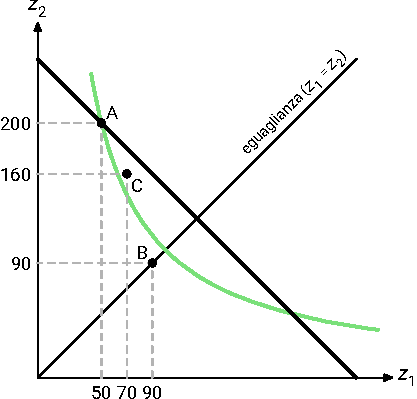
\includegraphics[width=\textwidth]{./figure/fbs-color-0.pdf}
\end{figure}
\end{column}
\end{columns}
\end{frame}


%%%%%%%%%%%%%%%%%%%%%%%%%%%%%%%%%%%%%%%%
\begin{frame}{Quanto siamo avversi alla diseguaglianza /2}
\begin{columns}
\begin{column}{.5\columnwidth}
\begin{itemize}
\item I punti A ed F hanno lo stesso reddito totale, ma in F c'è eguaglianza dei
redditi dei due individui
\item I punti A ed E sono equivalenti dal punto di vista sociale, ma in E il
reddito totale è inferiore (100,100) contro (250,40).
\item La forma convessa della curva riflette il grado di alla diseguaglianza
\end{itemize}
\end{column}

\begin{column}{.5\columnwidth}
\begin{figure}[htbp]
\centering
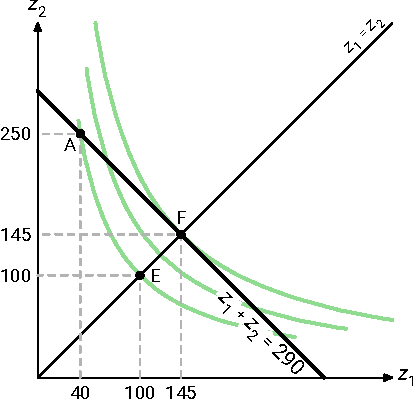
\includegraphics[width=\textwidth]{./figure/fbs-color-4.pdf}
\end{figure}
\end{column}
\end{columns}
\end{frame}

%%%%%%%%%%%%%%%%%%%%%%%%%%%%%%%%%%%%%%%%
\begin{frame}{Quanto siamo avversi alla diseguaglianza /3}
\begin{columns}
\begin{column}{.5\columnwidth}
\begin{itemize}
\item L'inclinazione della curva in un punto rappresenta quanto «peso» una
riduzione (aumento) del reddito di un individuo in rapporto a un aumento
(riduzione) del reddito dell'altro individuo:
\begin{itemize}
\item un incremento di 40 del reddito di 1, più povero, compensa (vale quanto)
una riduzione di 70 del reddito di 2, più ricco;
\item «pesiamo» 1€ del povero quanto 40/70=0,57€ del ricco.
\end{itemize}
\item Qui l'analogia è con il SMS nel caso della funzione di utilità.
\end{itemize}
\end{column}

\begin{column}{.5\columnwidth}
\begin{figure}[htbp]
\centering
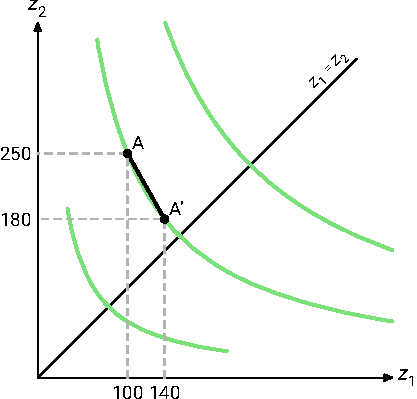
\includegraphics[width=\textwidth]{./figure/fbs-color-2.pdf}
\end{figure}
\end{column}
\end{columns}
\end{frame}


%%%%%%%%%%%%%%%%%%%%%%%%%%%%%%%%%%%%%%%%
\begin{frame}{Il costo della redistribuzione}
\begin{itemize}
\item Le politiche redistributive, ad es. le imposte dovute ma anche i sussidi
il cui importo dipende dal reddito, possono determinare un
costo per l'economia in quanto riducono gli incentivi degli individui a
produrre reddito.
\item Se un individuo ha 200 e l'altro 50, posso avvicinare i redditi dei due
individui introducendo un'imposta commisurata al reddito che finanzia un
trasferimento uniforme:
\begin{itemize}
\item es. imposta del 40\%
\begin{center}
\begin{tabular}{rrrr}
reddito iniziale & imposta & trasferimento & reddito finale\\[0pt]
\hline
200 & 80 & 50 & 170\\[0pt]
50 & 20 & 50 & 80\\[0pt]
\end{tabular}
\end{center}
\item ma l'imposta potrebbe disincentivare la produzione di reddito: 
\begin{center}
\begin{tabular}{rrrr}
reddito iniziale & imposta & trasferimento & reddito finale\\[0pt]
\hline
150 & 60 & 38 & 128\\[0pt]
40 & 16 & 38 & 62\\[0pt]
\end{tabular}
\end{center}
\end{itemize}
\end{itemize}
\end{frame}


%%%%%%%%%%%%%%%%%%%%%%%%%%%%%%%%%%%%%%%%
\begin{frame}{Il costo dell'imposta sul reddito da lavoro}
\begin{columns}
\begin{column}{.45\columnwidth}
\begin{itemize}
\item Gli individui traggono utilità dal consumo $x$ e sostengono un costo
(disutiltà) per ottenere un certo reddito $z$: $$x-\delta(z).$$ La funzione
$\delta(z)$ è crescente e convessa (produrre reddito diventa via via più costoso al
crescere di $z$).
\item Il costo (marginale e totale) di produrre reddito è maggiore per l'individuo
1: $\delta'_1(z)> \delta'_2(z)$ e $\delta_1(z)>\delta_2(z)$
\end{itemize}
\end{column}

\begin{column}{.45\columnwidth}
\begin{center}
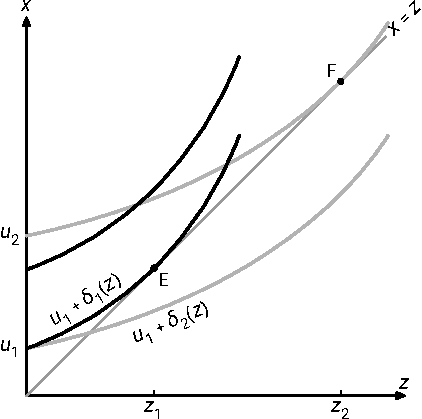
\includegraphics[scale=.8]{./figure/effetto-distorsivo-imposte-ql-1.pdf}
\end{center}

\begin{itemize}\small
\item E ed F rappresentano le scelte ottimali di $x$ e $z$ da parte dei due
individui in assenza di imposte.
\end{itemize}
\end{column}
\end{columns}
\end{frame}

%%%%%%%%%%%%%%%%%%%%%%%%%%%%%%%%%%%%%%%%
\begin{frame}{Introduciamo un'imposta sul reddito}
\begin{columns}[T]
\begin{column}{.55\columnwidth}
\begin{center}
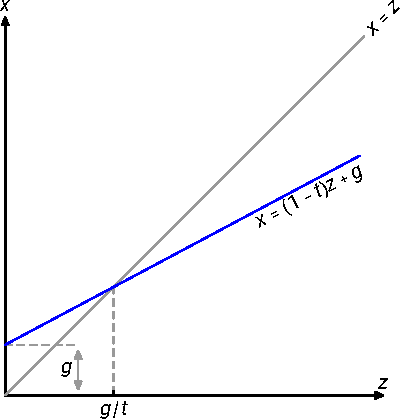
\includegraphics[scale=.9]{./figure/effetto-distorsivo-imposte-ql-color-2.pdf}
\end{center}
\end{column}


\begin{column}{.45\columnwidth}
\begin{itemize}
\item In assenza di imposte $x^i=z^i$
\item introducendo un'imposta lineare (proporzionale) sul reddito che finanzia un
trasferimento uniforme abbiamo: $x^i=(1-t)z^i+g$
\item deve essere soddisfatto il vincolo di bilancio fiscale: $n\cdot g=\sum_itz^i$
\end{itemize}
\end{column}
\end{columns}
\end{frame}

%%%%%%%%%%%%%%%%%%%%%%%%%%%%%%%%%%%%%%%%
\begin{frame}{Effetto dell'imposta/trasferimento sulle decisioni individuali}
\begin{columns}[T]
\begin{column}{.55\columnwidth}
\begin{center}
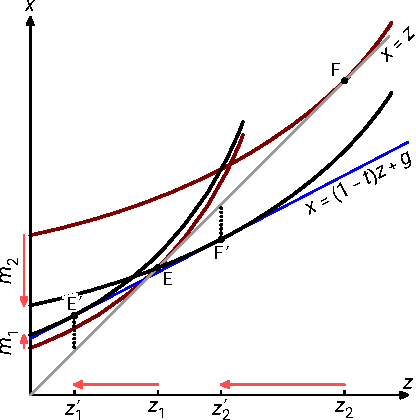
\includegraphics[scale=.9]{./figure/effetto-distorsivo-imposte-ql-color-3.pdf}
\end{center}
\end{column}


\begin{column}{.45\columnwidth}
\begin{itemize}
\item Dobbiamo modulare $g$ in modo da rispettare il vincolo di bilancio
fiscale (la distanza dei punti E' e F' dalla bisettrice rappresenta il
trasferimento netto ai due individui):
$$ (tz'_1-g)+(tz'_2+g)=0 $$
\item Nel nuovo equilibrio entrambi gli individui hanno ridotto il reddito
  prodotto da $z_i$ a $z'_i$;
\item le variazioni di utilità (misurate in unità monetarie di consumo) sono pari a $m_1$ e $-m_2$.
\end{itemize}
\end{column}
\end{columns}
\end{frame}

%%%%%%%%%%%%%%%%%%%%%%%%%%%%%%%%%%%%%%%%
\begin{frame}{La «perdita secca» dovuta all'effetto distorsivo dell'imposta}
\begin{columns}[T]
\begin{column}{.55\columnwidth}
\begin{center}
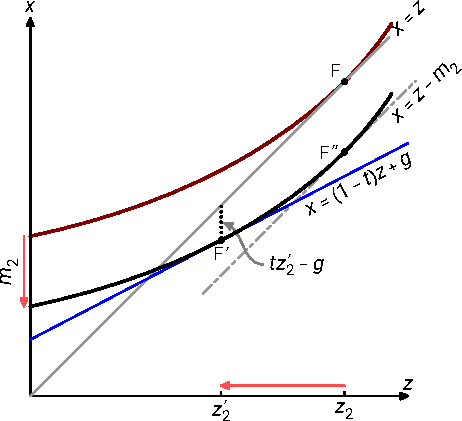
\includegraphics[scale=.9]{./figure/effetto-distorsivo-imposte-ql-color-4.pdf}
\end{center}
\end{column}


\begin{column}{.45\columnwidth}
\begin{itemize}
\item Supponiamo che all'individuo 2 fosse applicata un'imposta in somma fissa
  $m_2$ con effetti equivalenti in termini di utilità a quelli dello schema
  redistributivo ($tz_2-g$);
\item la differenza tra la riduzione equivalente del consumo $m_2$ e l'imposta
  netta $tz_2-g$ pagata dall'individuo rappresenta la «perdita secca» di
  benessere.
\end{itemize}
\end{column}
\end{columns}
\end{frame}


%%%%%%%%%%%%%%%%%%%%%%%%%%%%%%%%%%%%%%%%
\begin{frame}{Se avessimo avuto a disposizione imposte non distorsive}
\begin{columns}[T]
\begin{column}{.55\columnwidth}
\begin{center}
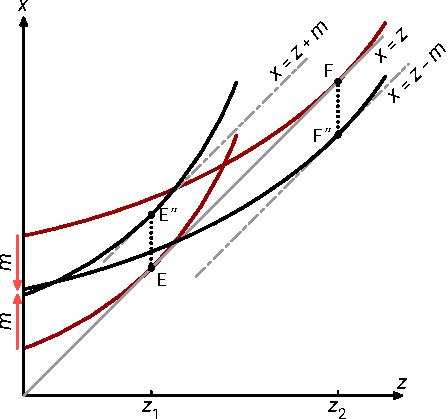
\includegraphics[scale=.9]{./figure/effetto-distorsivo-imposte-ql-color-5.pdf}
\end{center}
\end{column}

\begin{column}{.45\columnwidth}
  \begin{itemize}
\item Utilizzando imposte distorsive abbiamo $m_2>m_1$.
\item Se avessimo potuto trasferire reddito utilizzando \emph{imposte in somma fissa} di importo $m$ avremmo avuto un trasferimento 1:1, senza perdite.
\item L'imposta in somma fissa (= il cui ammontare è fisso al variare del comportamento dell'individuo) è un'imposta che non produce effetto distorsivo, ha solo un effetto \emph{di reddito}.
\end{itemize}
\end{column}
\end{columns}
\end{frame}

%%%%%%%%%%%%%%%%%%%%%%%%%%%%%%%%%%%%%%%%
\begin{frame}{Ottimo sociale con imposte distorsive}
\begin{columns}
\begin{column}{.55\columnwidth}
\begin{center}
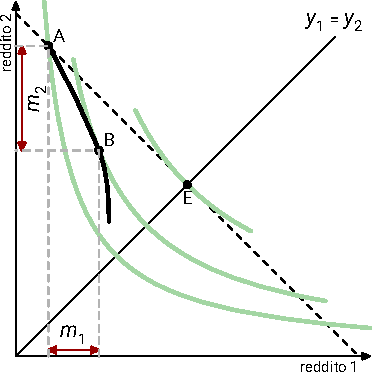
\includegraphics[width=\textwidth]{./figure/fbs-color-6.pdf}
\end{center}
\end{column}


\begin{column}{.45\columnwidth}
\begin{itemize}
\item La necessità di ricorrere a imposte distorsive impedisce di muoversi lungo la retta inclinata di 45°, ci costringe a spostarci su un punto inferiore (\emph{second best});
\item l'ottimo \emph{trade-off} tra equità ed efficienza dipende dalla nostra propensione a redistribuire e dall'entità dell'effetto distorsivo.
\end{itemize}
\end{column}
\end{columns}
\end{frame}


%%%%%%%%%%%%%%%%%%%%%%%%%%%%%%%%%%%%%%%%
\begin{frame}{Da cosa dipende la dimensione della distorsione?}
\begin{columns}
\begin{column}{.55\columnwidth}
\begin{center}
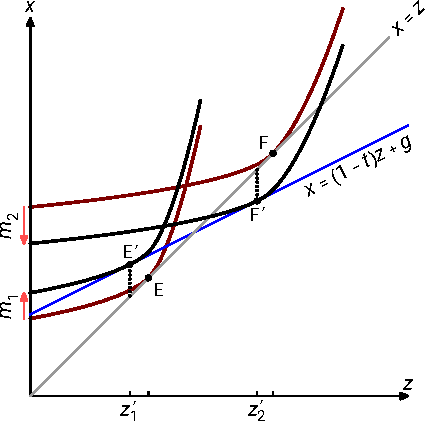
\includegraphics[width=\textwidth]{./figure/effetto-distorsivo-imposte-ql-color-8.pdf}
\end{center}
\end{column}


\begin{column}{.45\columnwidth}
\begin{itemize}
\item L'entità dell'effetto distorsivo dipende dalla dimensione dell'effetto di sostituzione;
\item tale effetto dipende dalla «curvatura» (grado di convessità) delle curve di indifferenza: quanto varia il reddito $z^i$ a fronte di variazioni dell'inclinazione del vincolo di bilancio.
\item Esistono imposte prive di effetti distorsivi?
\end{itemize}
\end{column}
\end{columns}
\end{frame}

%%%%%%%%%%%%%%%%%%%%%%%%%%%%%%%%%%%%%%%%
\begin{frame}{Da cosa dipende la dimensione della distorsione? /2}
\begin{itemize}
\item L'effetto distorsivo dipende da quanto il reddito reagisce alla
  variazione dell'imposta (tenendo conto dell'effetto indiretto determinato da
  $g$, che è un effetto di reddito).
\item Viene comunemente misurato dall'elasticità:
  \begin{equation*}
 e = -\dfrac{dz}{d(1-t)}\dfrac{1-t}{z}.
\end{equation*}

\item N.B. Invece di $t$ si preferisce considerare come variabile $(1-t)$, il
  cui valore è proporzionale al reddito ed esprime direttamente l'inclinazione
  del vincolo di bilancio.
\item Molte analisi econometriche hanno cercato di determinare $e$, ma il suo
  valore resta ampiamente dibattuto tra gli economisti.
\end{itemize}
\end{frame}

%%%%%%%%%%%%%%%%%%%%%%%%%%%%%%%%%%%%%%%%
\begin{frame}{La curva di Laffer}
\begin{itemize}
\item Immaginiamo di voler massimizzare il gettito $t(z_1+z_2)=t\bar{z}$, ovvero di voler
massimizzare $g$
\item Derivando abbiamo:
\begin{equation*}
  \frac{dg}{dt}=\bar{z}-t\frac{d\bar{z}}{d(1-t)} = \bar{z}\left(1-\frac{t}{1-t}\frac{d\bar{z}}{d(1-t)}\frac{1-t}{\bar{z}}\right)=
  \bar{z}\left(1-\frac{t}{1-t}e\right)
\end{equation*}
dove $t/(1-t)$ aumenta all'aumentare di $t$.
\end{itemize}

\begin{columns}
\begin{column}{.45\columnwidth}
\begin{center}
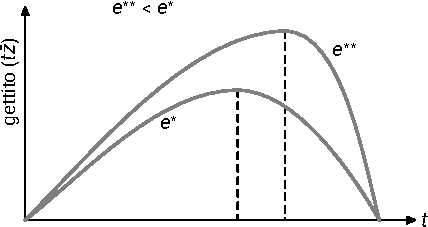
\includegraphics[width=\textwidth]{./figure/laffer-1.pdf}
\end{center}
\end{column}

\begin{column}{.45\columnwidth}
\begin{itemize}
\item Se $e$ non si riduce all'aumentare di $t$, vi sarà un punto dove $dg/dt$ diventa negativa;
\item $dg/dt=0$ implica $t=\frac{1}{1+e}$.
\end{itemize}
\end{column}
\end{columns}
\end{frame}

\section{Come redistribuire}


%%%%%%%%%%%%%%%%%%%%%%%%%%%%%%%%%%%%%%%%
\begin{frame}{L'effetto redistributivo delle imposte e spesa pubblica /1}
\begin{itemize}
\item Contributi e benefici netti del quintile superiore e inferiore (dati riferiti a metà anni 2000)
\end{itemize}

\begin{center}
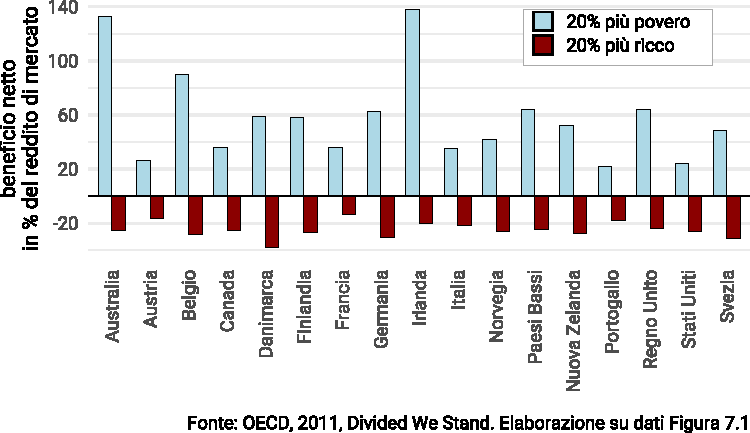
\includegraphics[width=.9\textwidth]{./figure/effetti-redistributivi-imposte-benefici-color.pdf}
\end{center}
\end{frame}

%%%%%%%%%%%%%%%%%%%%%%%%%%%%%%%%%%%%%%%%
\begin{frame}{L'effetto redistributivo delle imposte e spesa pubblica /2}
\begin{itemize}
\item Confronto tra diseguaglianza del reddito di mercato e reddito disponibile
\item Riferimento all'indice di concentrazione di Gini
\end{itemize}

\begin{center}
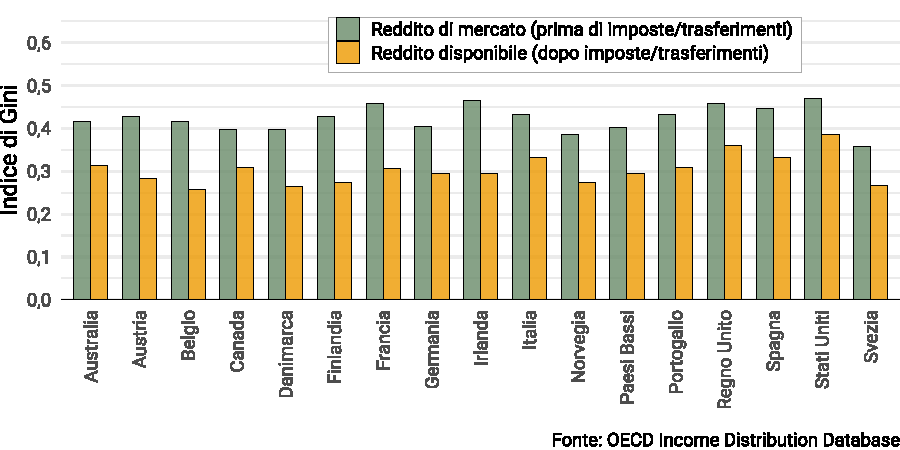
\includegraphics[width=\textwidth]{./figure/gini-mkt-disp-color.pdf}
\end{center}
\end{frame}

%%%%%%%%%%%%%%%%%%%%%%%%%%%%%%%%%%%%%%%%
\begin{frame}{L'effetto redistributivo delle imposte e spesa pubblica /3}
Qualche avvertenza:
\begin{itemize}
\item queste misurazioni non riescono a tenere conto in modo adeguato dei beni e servizi in natura (istruzione, sanità, beni pubblici);
\item la redistribuzione può influenzare anche il reddito di mercato, aumentando la diseguaglianza (es. pensioni, sostegno alla maternità) o più probabilmente riducendola (sanità, istruzione, ecc.);
\item si parla a volte di \alert{predistribuzione} per indicare le politiche che incidono sulla distribuzione del reddito prima delle imposte.
\end{itemize}
\end{frame}

%%%%%%%%%%%%%%%%%%%%%%%%%%%%%%%%%%%%%%%%
\begin{frame}{Le forme della redistribuzione sul lato della spesa}
Trasferimenti universali o selettivi?
\begin{itemize}
\item Selettivi: prova dei mezzi (\emph{means-tested}).
\item Universalismo coerente con il riconoscimento di diritti sociali.
\item Possibile effetto «stigma» se prestazioni legati a condizione di indigenza.
\item Maggiore complessità amministrativa dei programmi selettivi.
\item I programmi universalistici sono realmente più costosi?\\[0pt]
Esempio:
\begin{itemize}
\item Caso 1: 3 individui con reddito 50, 30 e 10. Imposta 30\%.
\item Caso 2: imposta pagate solo dai più ricchi $0,3(z-30)$, benefici in funzione del reddito $g(z)=9-0,3z$.
\end{itemize}
\item I programmi selettivi potrebbero andare incontro nel tempo a un'erosione
del consenso politico.
\end{itemize}
Trasferimenti monetari o «in natura»?
\end{frame}
\end{document}